\documentclass[a4paper,11pt]{article}

% Packages
\usepackage[utf8]{inputenc}
\usepackage[margin=1in]{geometry}
\usepackage{amsmath, amssymb}
\usepackage{eso-pic}
\usepackage{graphicx}
\usepackage{transparent}
\usepackage{helvet}
\usepackage{multicol}
\usepackage{xcolor}

% BACKGROUND IMAGE
\begin{document}
\AddToShipoutPictureBG*{
\AtPageLowerLeft{\transparent{0.6}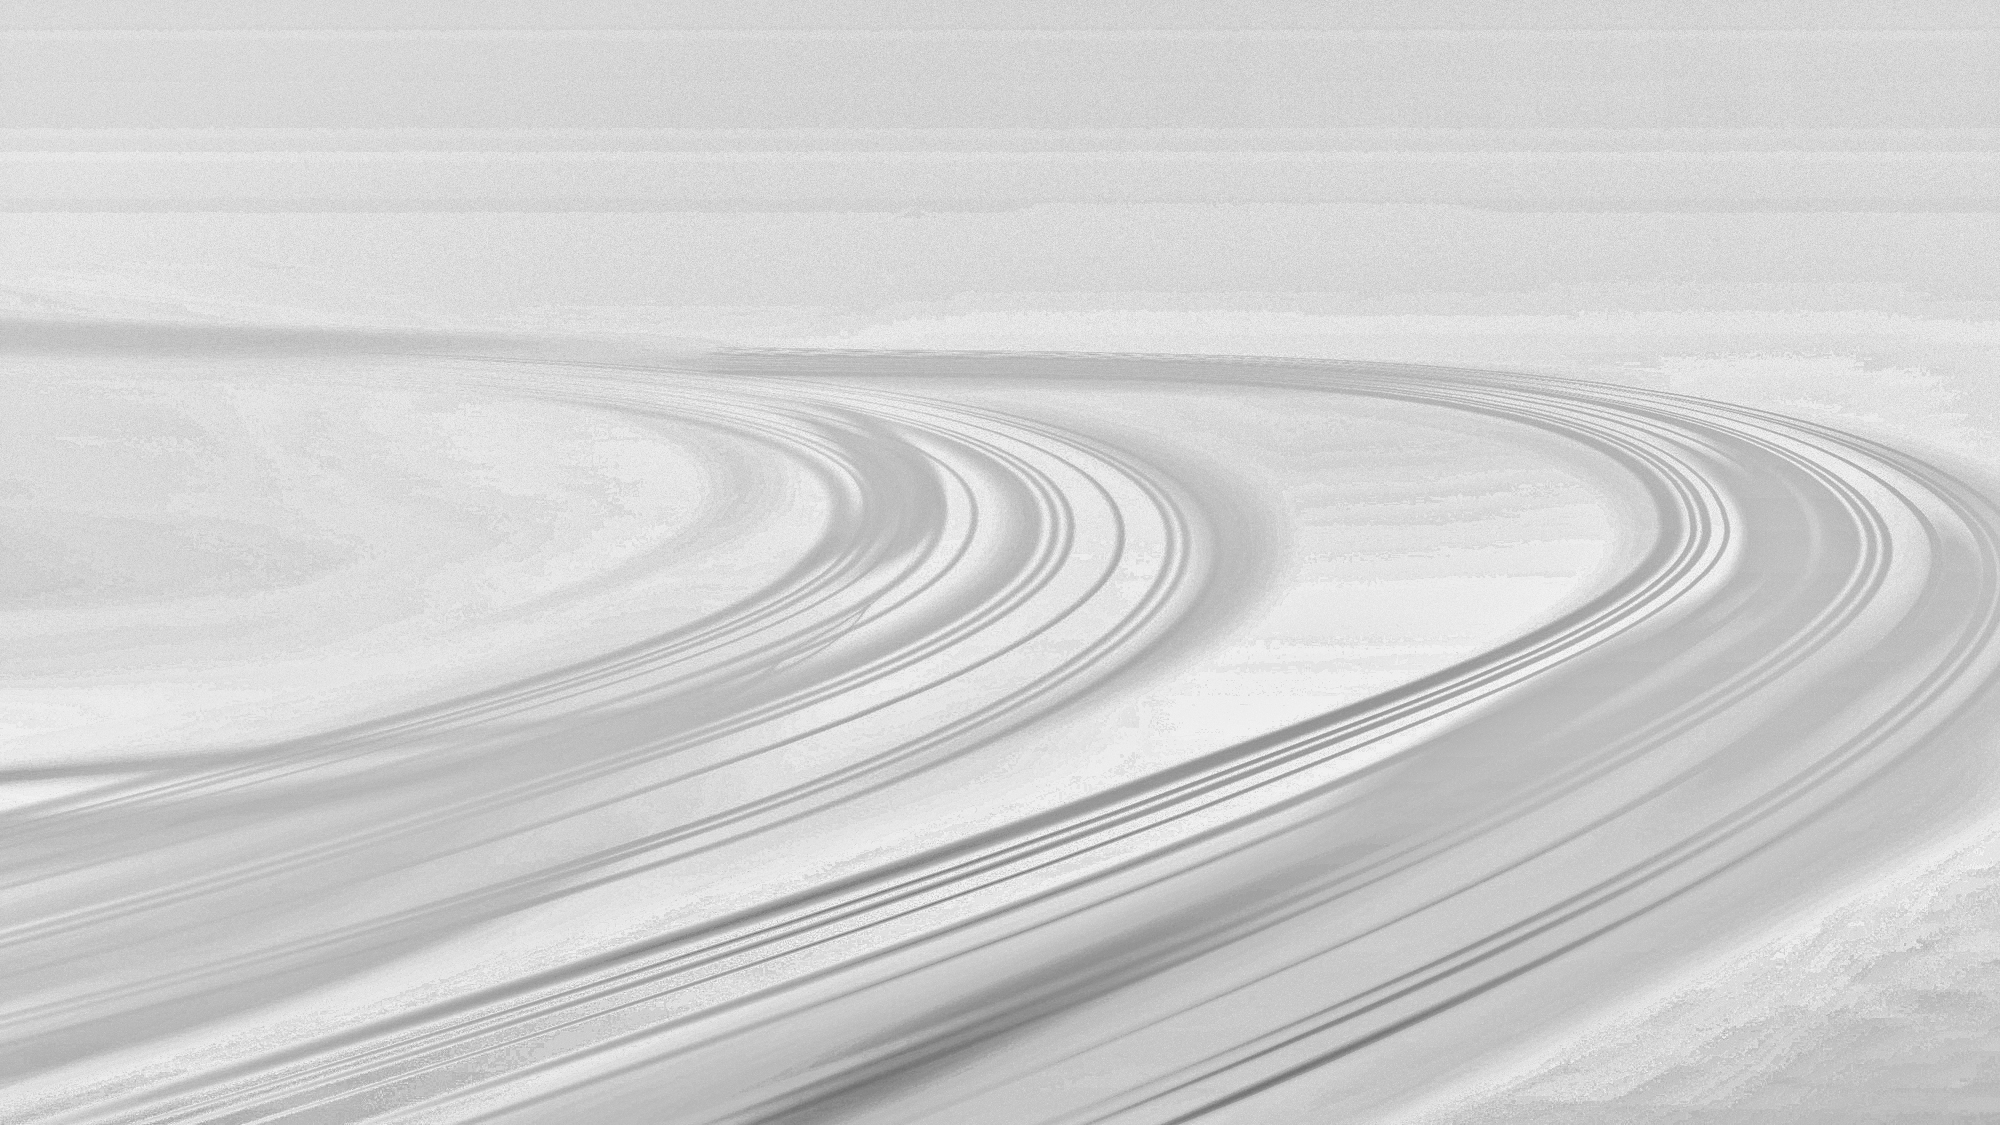
\includegraphics[width=\paperwidth,height=\paperheight]{template-art/Nat/NatTitle_BW.jpg}
    }
}

% NAT FAK LOGO
\begin{figure}[t]
    \centering
    
\includegraphics[width=0.7 \textwidth]{template-art/Nat/NatKennung.pdf}
    \label{fig:natfaklogo}
\end{figure}

% TITLE PAGE
\pagenumbering{roman} %I want roman numerals for the title page and index, but not for the main content. So I set it to roman here, and then switch to arabic later.
\begin{center}
    \vspace*{\fill}
     {\large {Experiment Nr. 31}}
     \\[0.3cm]
    % Title
    \textcolor[RGB]{90,180,50}{\fontsize{46}{0}\selectfont \textbf{\textsf{Superconductivity}}}
    \\[0.3cm]
    {\Large \textbf{Date of Submission: \today \\\vspace{0.2cm} Group Nr. M602}}\\
      \vspace*{\fill}
    
      % Authors
    {\Large
    \begin{tabular}{c @{\hspace{2cm}} c}
        Pravin Mani Kannan & Barathraj Radhakrishnan Subramanian \\
        Mat. Nr: 23459332 & Mat. Nr: idk
    \end{tabular}} \\[1cm]

  
\end{center}
 % Bottom spring

\begin{figure}[b]
    \centering
    
\includegraphics[width=0.3 \textwidth]{template-art/FAUWortmarkeBlau.pdf}
    \label{fig:nat}
\end{figure}


\newpage{} % INDEX
\tableofcontents

\newpage % Start of main content

\pagenumbering{arabic}


\section{Introduction}

\section{Electrical Resistance and Temperature Dependence}
    \subsection{Metals}
    \subsection{Semiconductors}
    \subsection{Superconductors and BCS Theory}

\section{Magnetic Properties of Superconductors}
    \subsection{Ideal Diamagnetism and the Meissner Effect}
    \subsection{Type-I vs. Type-II Superconductors}
    \subsection{Flux Quantization and Abrikosov Vortex Lattice}

\section{Magnetic Susceptibility and Magnetization}
    \subsection{Diamagnetic, Paramagnetic, and Ferromagnetic Materials}
    \subsection{Magnetization Curves of Superconductors}
    \subsection{Critical Field, Temperature, and Current Density}

\section{Experimental Methods}
    \subsection{Four-Point Probe Measurements}
    \subsection{Inductive AC-Susceptibility Measurements}
    \subsection{Deep-Stick Setup and Lock-In Technique}

\section{Conclusion}

\end{document}